\chapter{Architectural Design}
This section aims to present and analyze the architecture of the S2B in a top-down manner. 
We discuss about the architectural design choices and the reasons behind them. 

\section{Overview: High-level components and their interactions}
The figure shown below represents a high-level description of the components which make up the system.
\begin{figure}[H]
    \centering
    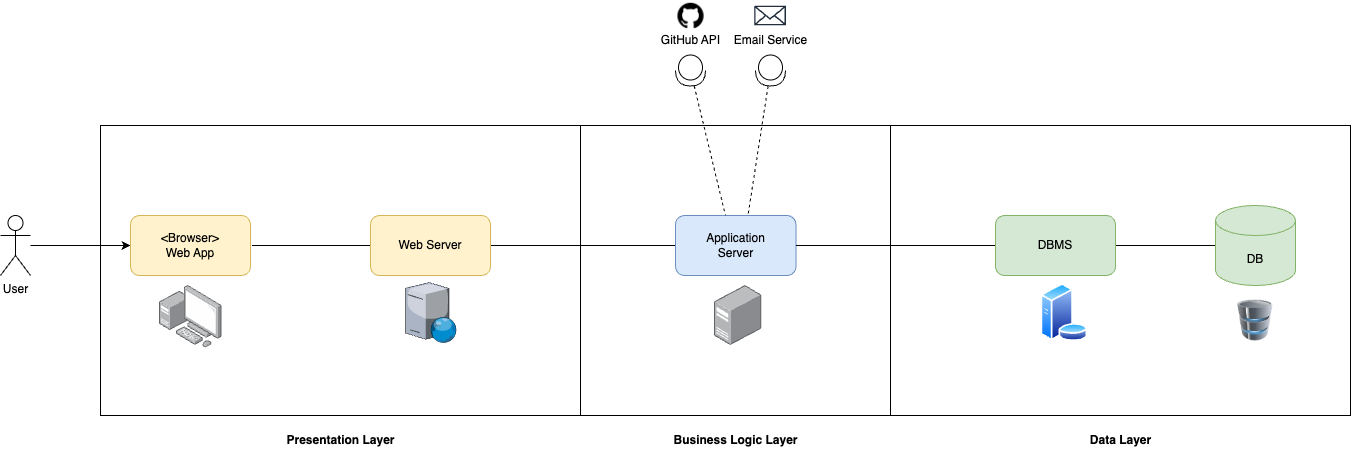
\includegraphics[width=\textwidth]{images/component_view/high_level.png}
    \caption{Overview CKB architecture}
    \label{fig:CKB Architecture}
\end{figure}
A web interface will be used to access the platform. 
The overall architecture of the system is based on a three-tier architecture, 
with the application servers interacting with a database management system and
using APIs to retrieve and store data. \\
The three logical layers corrspond to three different physical layers and each layer can communicate only with the adjacent ones.
The interactions between clients and server are stateless according to the REST architectural style. \\
The web server is responsible for the communication with the clients and for the management of the requests. \\
The application server holds the business logic of the application and it can communicate with the database server to retrieve and store data, also with the GitHub platform and the Email Service. 

\section{Component view}

\subsection{High level view}
\begin{figure}[H]
    \centering
    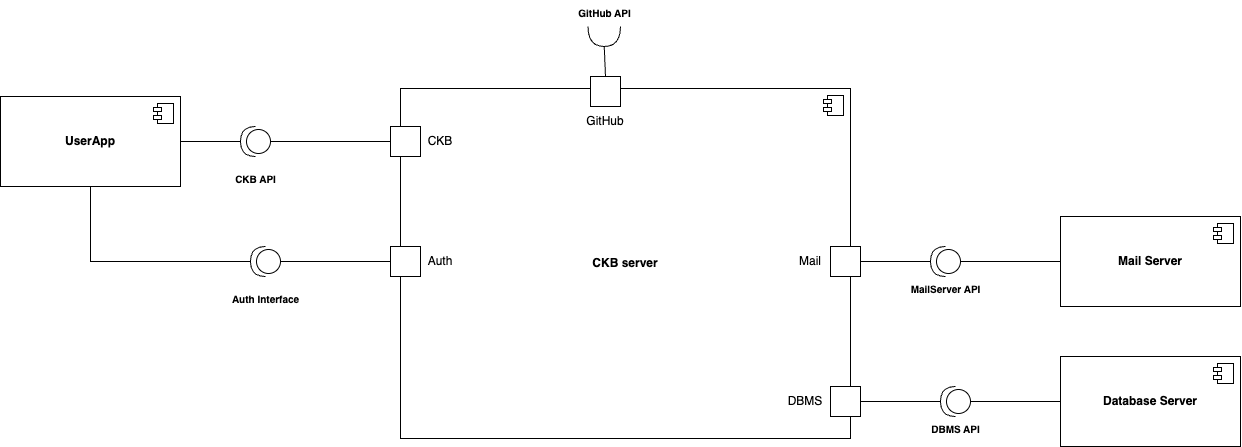
\includegraphics[width=\textwidth]{images/component_view/Component_view.png}
    \caption{High level component view}
\end{figure}
The figure above shows the system components and interfaces at a high level.
\begin{itemize}
    \item \textbf{CKB Server: } it represents the core of the CKB system and it contains all the business logic.
    \item \textbf{UserApp: } it represents the web application used by the users to access the CKB platform. Users register and log into the system through the 
    \textbf{Auth interface} and access the functionalities offered by the system through the \textbf{CKB API}.
    \item \textbf{Database Server: } it represents the DBMS used to store the data of the system. The system can access the data through the \textbf{DBMS API}.
    \item \textbf{Mail Server: } it represents the mail server used to send notifications to the users. The system can access the mail server through the \textbf{MailServer API}.
\end{itemize}

\subsection{CKB Server detailed view}
\begin{figure}[H]
    \centering
    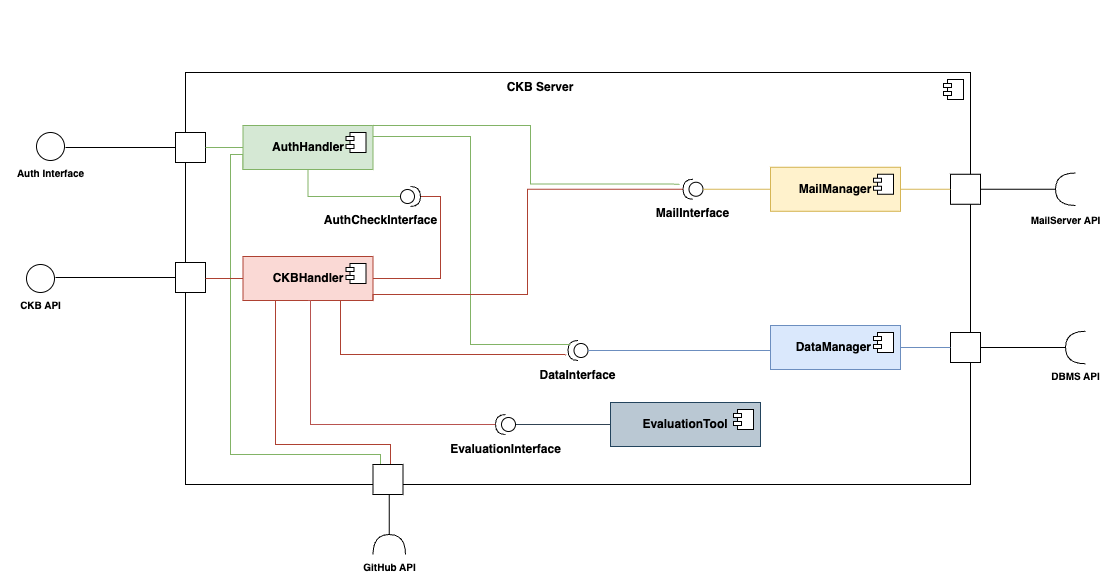
\includegraphics[width=\textwidth]{images/component_view/CKB_component.png}
    \caption{CKB server component view}
\end{figure}
The figure above shows the internal componenents of the CKB server.
\begin{itemize}
    \item \textbf{AuthHandler: } it handles the login and registration of the users. It offers the \textbf{AuthCheckInterface} to allow other components to check 
    if a user is authorized. It communicates with the \textbf{MailInterface} to manage confirmation emails and with the \textbf{DataInterface} to check the credentials
    correctness.
    \item \textbf{CKBHandler: } it handles all the functionalities offered by the system. It communicates with the \textbf{DataInterface} to retrieve and store data, with 
    the \textbf{AuthCheckInterface} to check if a user is authorized to perform a certain operation and with the \textbf{MailInterface} to send notifications to the users.
    It also communicates with the \textbf{GitHubInterface} to retrieve data (nickname and pushed code) from the GitHub platform.
    \item \textbf{MailManager: } it handles the access to the mail server, it provides the \textbf{MailInterface} that allows components to send emails.
    \item \textbf{DataManager: } it handles the access to the persistent data saved on the DB, almost every component communicates with it through the \textbf{DataInterface}.
    \item \textbf{EvaluationTool: } it handles the evaluation of the students' code based on the battle rules. It retrieves this information from the \textbf{CKBHandler}.
\end{itemize}


\subsection{Auth component view}
\begin{figure}[H]
    \centering
    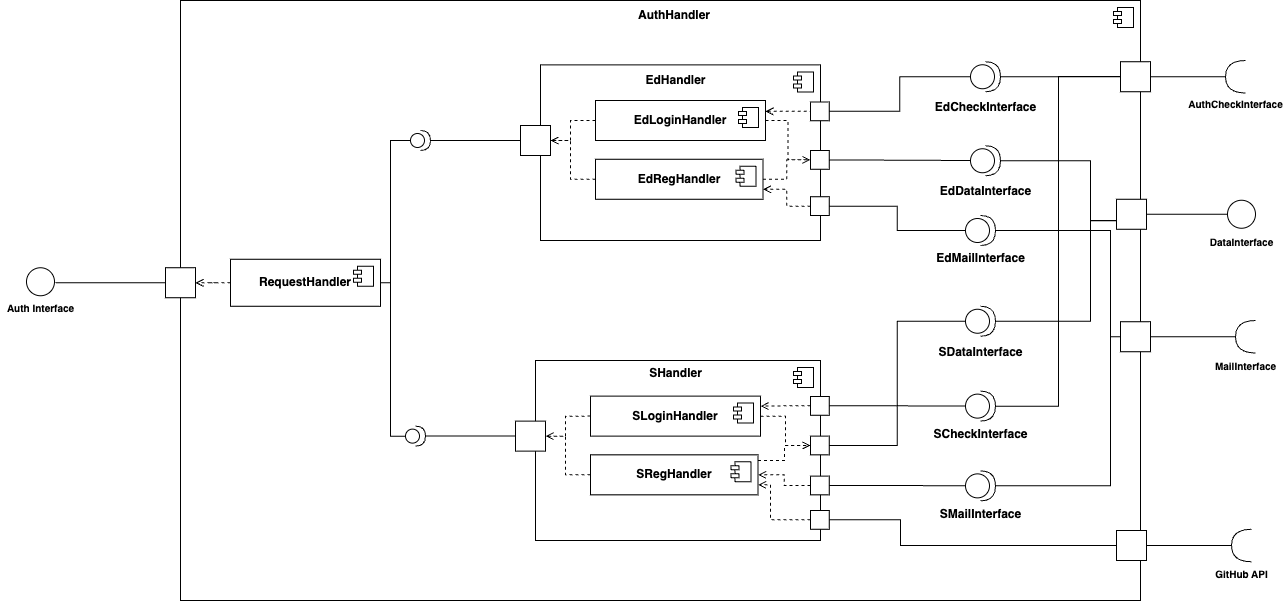
\includegraphics[width=\textwidth]{images/component_view/Auth.png}
    \caption{Auth component view}
\end{figure}
The figure above shows the internal componenents of the AuthHandler.
\begin{itemize}
    \item \textbf{RequestHandler: } it handles the requests acting as a router dispatching requests to the right handler.
    \item \textbf{EdHandler: } it is composed by the \textbf{EdLoginHandler} and the \textbf{EdRegHandler}. The former handles the login of educators, 
    the latter handles their registration.
    \item \textbf{SHandler: } it is composed by the \textbf{SLoginHandler} and the \textbf{SRegHandler}. The former handles the login of students,
    the latter handles their registration.
\end{itemize}
LoginHandlers communicate with the \textbf{AuthCheckInterface} to check the authorization of a user.\\
RegistrationHandlers communicate with the \textbf{MailInterface} to send confirmation emails and with the \textbf{DataInterface} to store the data of the new user.\\
SRegistrationHandler also communicate with \textbf{GitHubAPI} to link the CKB account with the GitHub one.

\section{Deployment view}
The figure below shows the architecture of the system. All the users access to the WebApp through the browser, which communicate with
the Web Server. Both Web Server and Application Server are hosted on a Cloud Provider. This choice offers many
advantages, such as:

\begin{itemize}
    \item  \textbf{Scalability and flexibility: }the ability of adding and removing resources efficiently throw 
    the use of load balancing services which allows the application server to manage traffic and workload. 
    \item   \textbf{Security: }the ability to protect the application server using firewall and DMZ, againist cyberattacks and possible threats.
    \item   \textbf{Cost efficiency:} the ability to pay only for the resources used which can help to lower the overall cost. 
\end{itemize}

\begin{figure}[H]
    \centering
    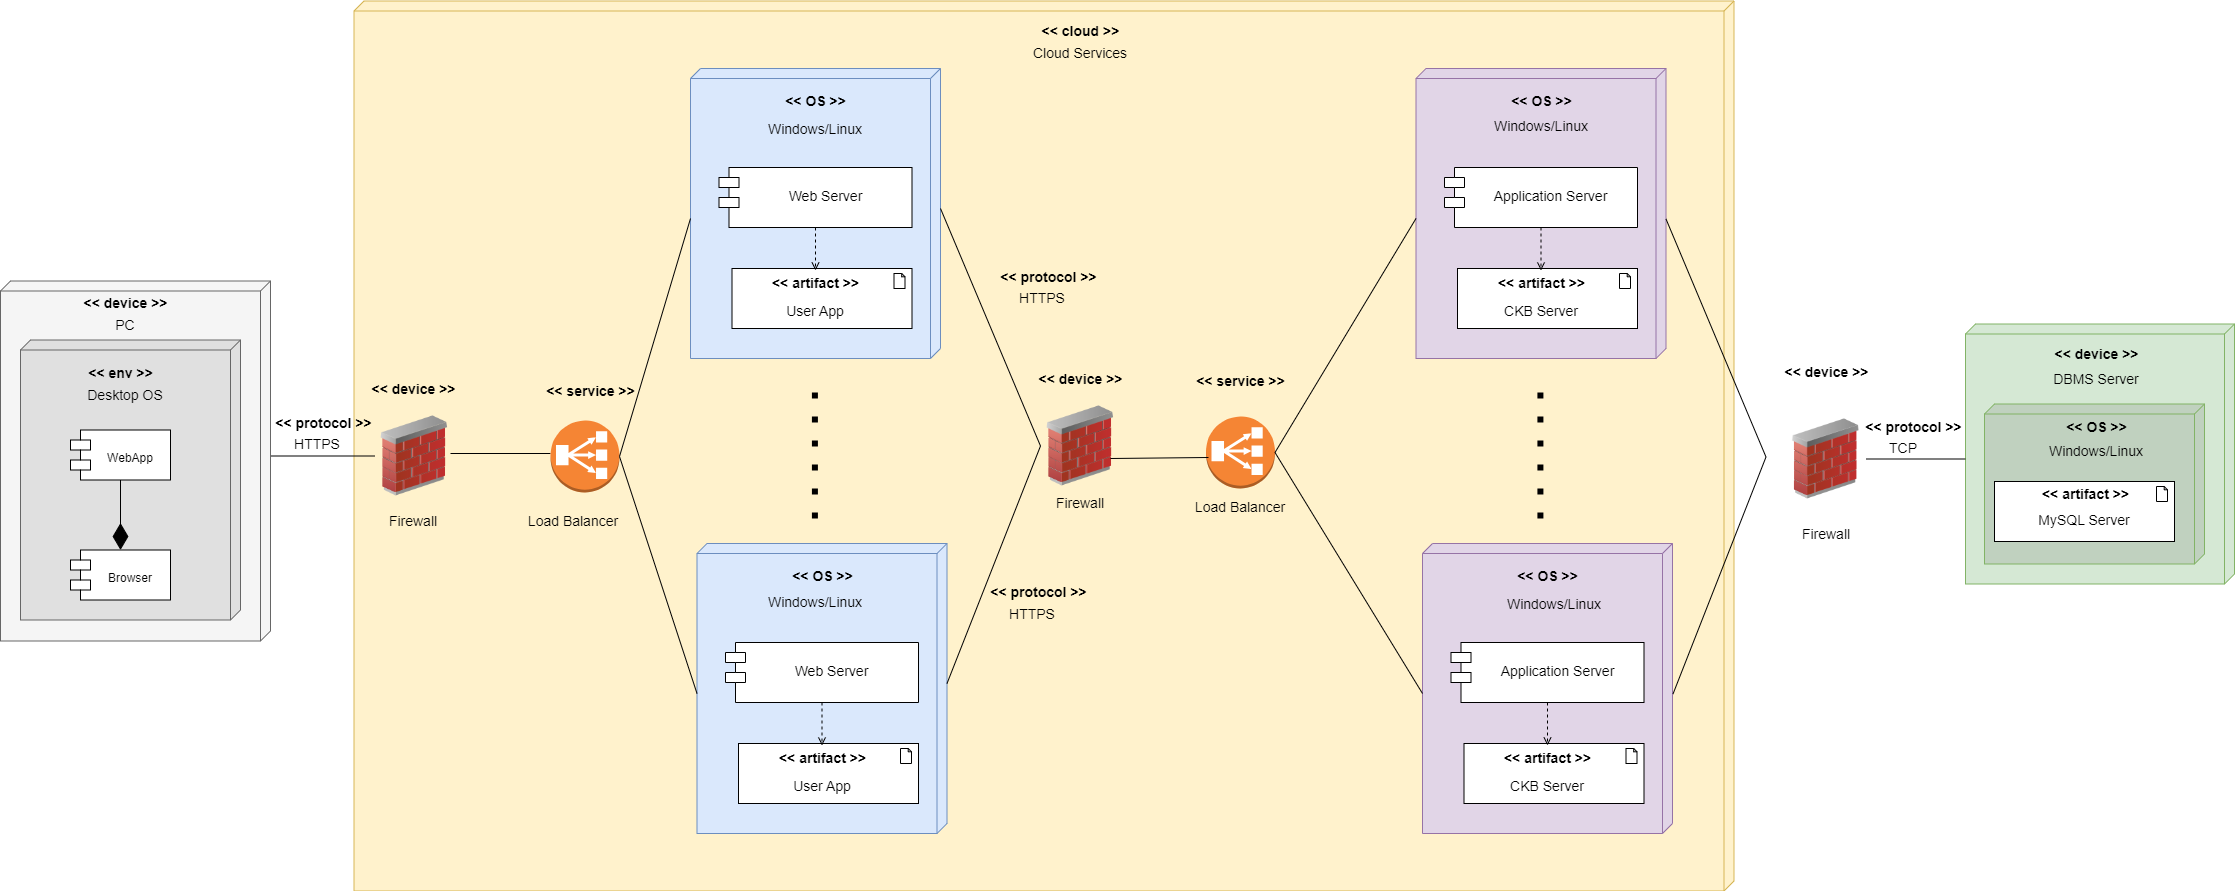
\includegraphics[width=1\textwidth]{images/Deployment_diagram.png}
    \caption{Deployment diagram}
\end{figure}

The deployment diagram offers a more detailed view over the hardware and software components of the system. 
\begin{itemize}
    \item  \textbf{PC: }is any device having a browser capable of running the JavaScript code.
    \item   the Cloud Services will host all the business and data logic for the system. It is characterized by 
    \begin{itemize}
        \item  \textbf{Firewall:} devices are used to protect and filter incoming connections to the logic and data layers of the system. It protects the system from unauthorized access and malicious attacks.
        \item  \textbf{Load Balancer:} services are used to distribute the workload across multiple servers. It helps to improve the performance and reliability of the system. It also helps to ensure that application can handle a large volume of requests, without any downtime.
        \item  \textbf{Multiple copies of Web Server and Application Server:} are used to ensure that the system is always available. The different instances can be created and destroyed dynamically, based on the workload. It also helps to achieve fault tolerance by allowing traffic to be redirect to a different instance, if one instance becomes unavailable.
    \end{itemize}
    \item   \textbf{Database:} is used to store all the data of the system. It uses MySQL as DBMS to retrieve and store data.
    \item   \textbf{Mail Provider: }is used to send notifications to the users. It uses Gmail as mail provider.
\end{itemize}

\section{Runtime view}
\subsection{Registration Student}
The figure below shows the sequence diagram of the registration of a student. The student compiles the form with his email and password and submits it. 
The database checks if the email is already used, if not the system sends a confirmation email to the student to complete the registration. 
The student inserts his personal information (name, surname, date of birth) and also his GitHub nickname. 
The system checks if the GitHub nickname is valid, if yes the system saves the student credentials and the registration is completed.

\begin{figure}[H]
    \centering
    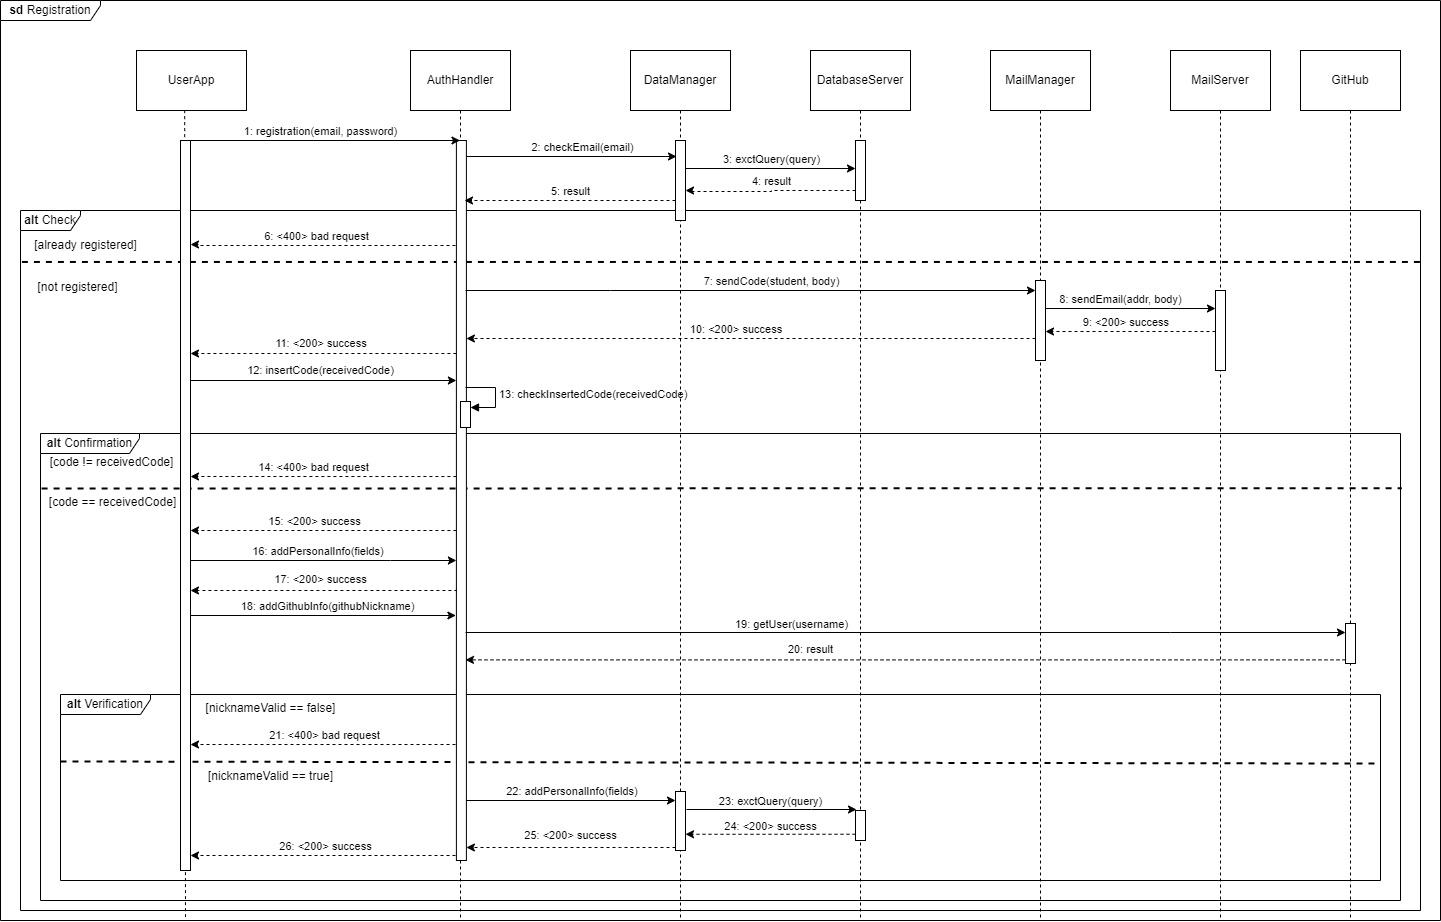
\includegraphics[width=1\textwidth]{images/seq_diagrams/RegistrationStd_DD.png}
    \caption{Registration Student}
\end{figure}

\subsection{Registration Educator}
The figure below shows the sequence diagram of the registration of an educator. The educator compiles the form with his email and password and submits it. 
The database checks if the email is already used, if not the system sends a confirmation email to the educator to complete the registration. 
The educator inserts his personal information (name, surname, date of birth) and the system saves the educator credentials and the registration is completed.
\begin{figure}[H]
    \centering
    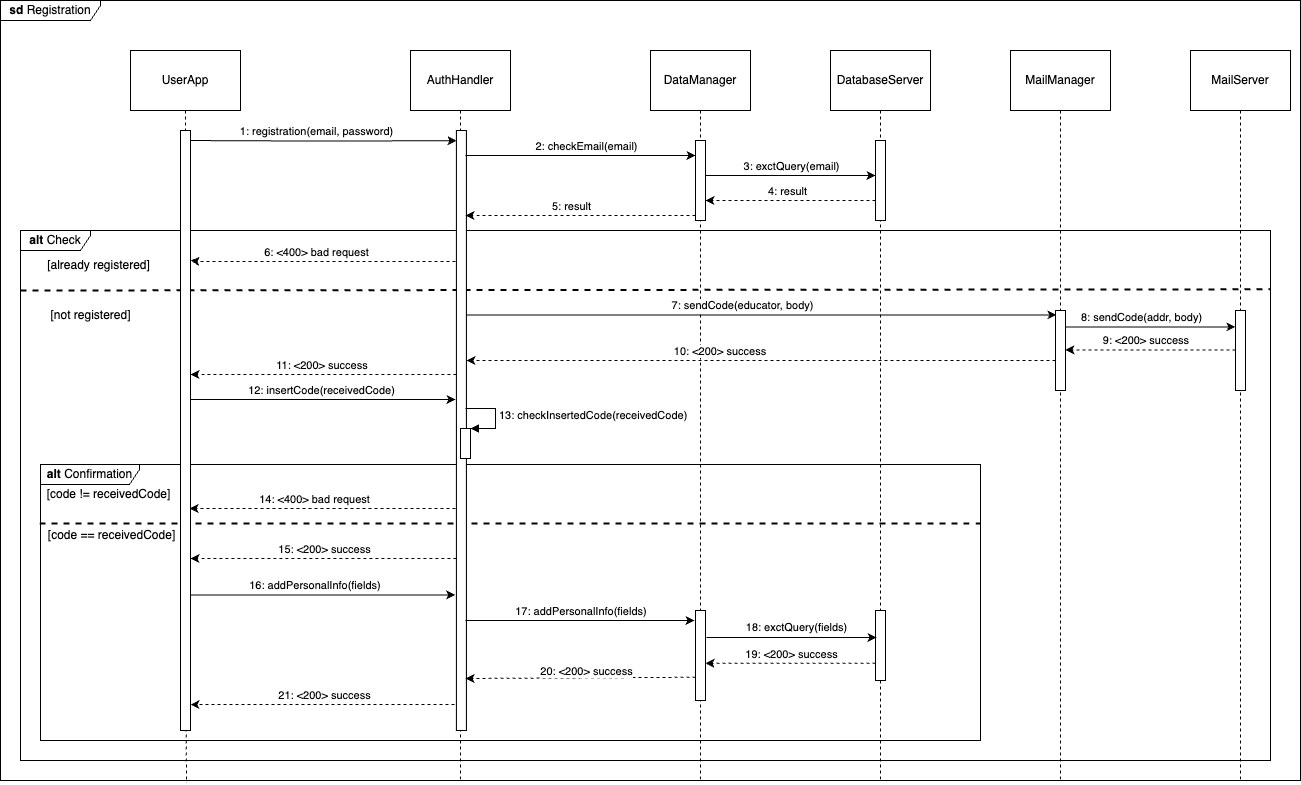
\includegraphics[width=1\textwidth]{images/seq_diagrams/RegistrationEd_DD.png}
    \caption{Registration Educator}
\end{figure}

\subsection{Login}
The figure below shows the sequence diagram of the user login. The user compiles the form with his email and password and submits it. 
The system checks if the credentials are stored and valid, if yes the user is logged in, otherwise the system shows an error message.
\begin{figure}[H]
    \centering
    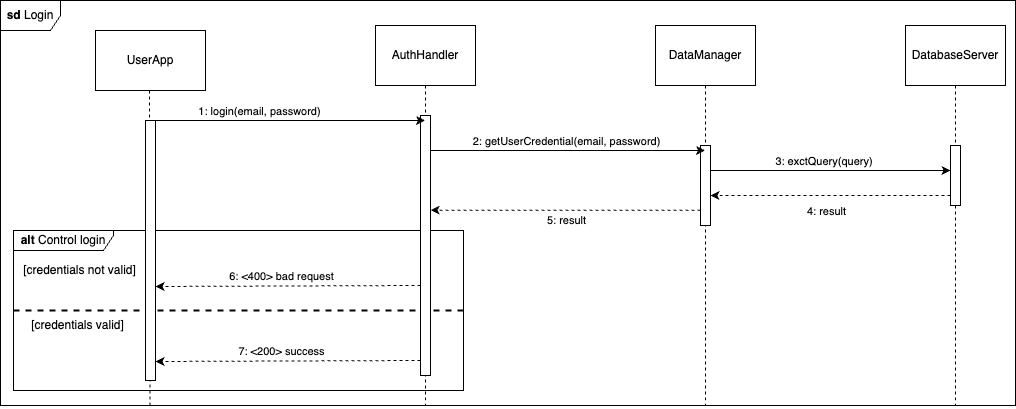
\includegraphics[width=1\textwidth]{images/seq_diagrams/Login_DD.png}
    \caption{Login}
\end{figure}

\subsection{Creation of the tournament}
The figure below shows the sequence diagram of the creation of a tournament. The educator compiles the form
 with the tournament details and submits it. The system checks if the data are valid, and if the badge option is set to true, the system creates the badge.
 After that the system send an email to all the granted colleagues. The tournament is created and the educator is redirected to the tournament page.

 \begin{figure}[H]
    \centering
    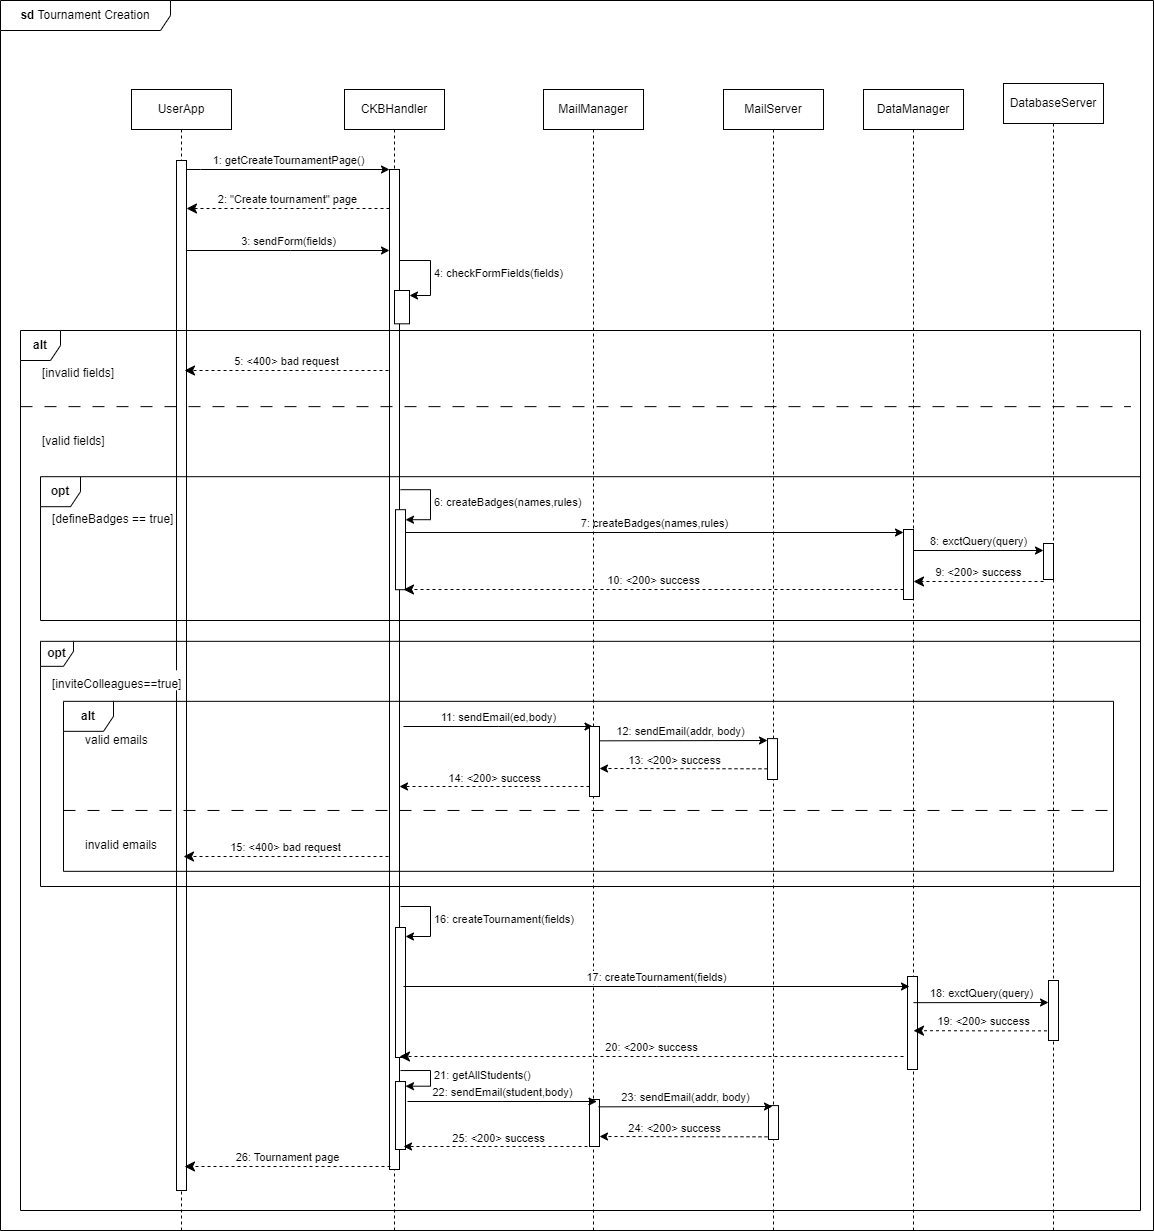
\includegraphics[width=1\textwidth]{images/seq_diagrams/tournament_creation_DD.png}
    \caption{Creation of the tournament}
\end{figure}

\subsection{Creation of the battle}
The figure below shows the sequence diagram of the creation of a battle. After the educator clicked ok the "Create Battle" button, he compiles the form
 with the battle details and submits it. The system checks if the data are valid. The battle is created, so the system send an email to all 
 the submitted students.  
 
\begin{figure}[H]
    \centering
    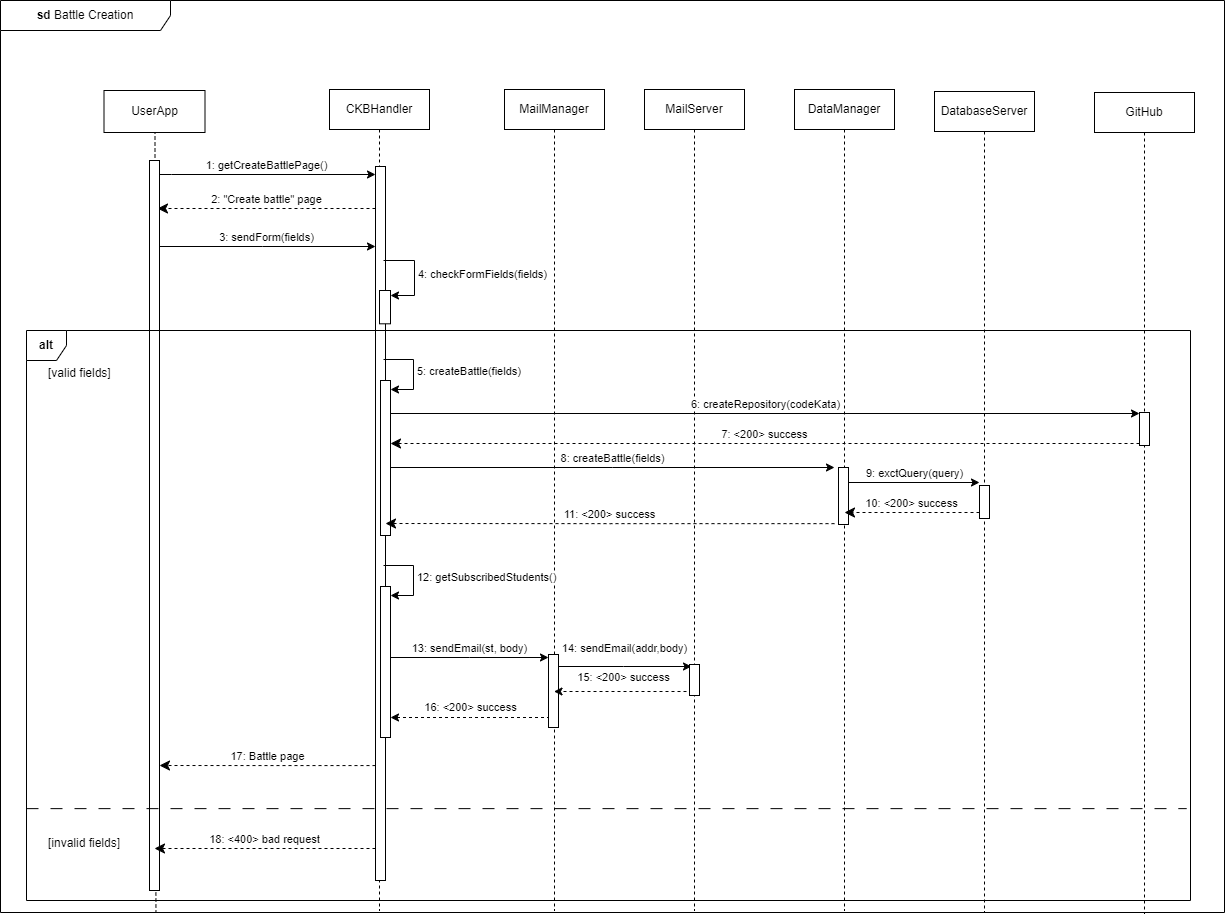
\includegraphics[width=1\textwidth]{images/seq_diagrams/battle_creation_DD.png}
    \caption{Creation of the battle}
\end{figure}

\subsection{Tournament visualization}
The figure below shows the sequence diagram of the visualization of a tournament. First the user requests the list of ongoing tournaments, 
then the user selects the tournament he wants to visualize.\\
\begin{figure}[H]
    \centering
    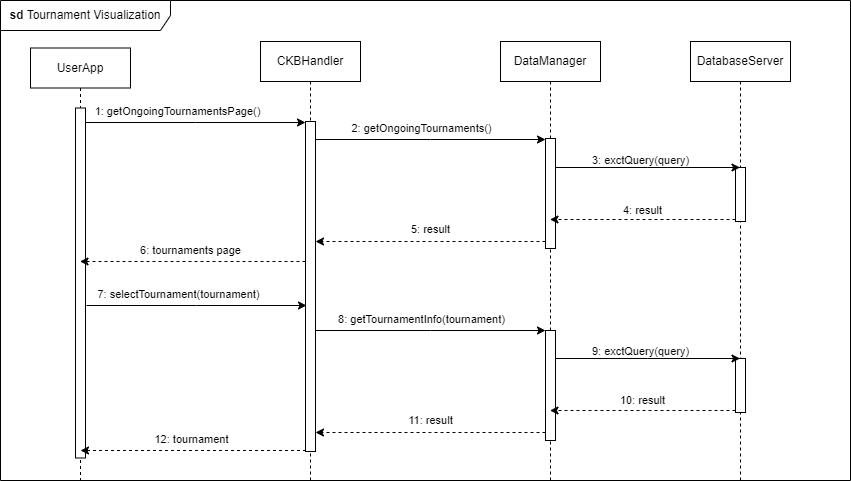
\includegraphics[width=1\textwidth]{images/seq_diagrams/tournament_visualization_dd.png}
    \caption{Tournament visualization}
\end{figure}

\subsection{Joining a tournament}
The figure below shows how a student can sign up for a tournament and receive an email notification about it.\\
\begin{figure}[H]
    \centering
    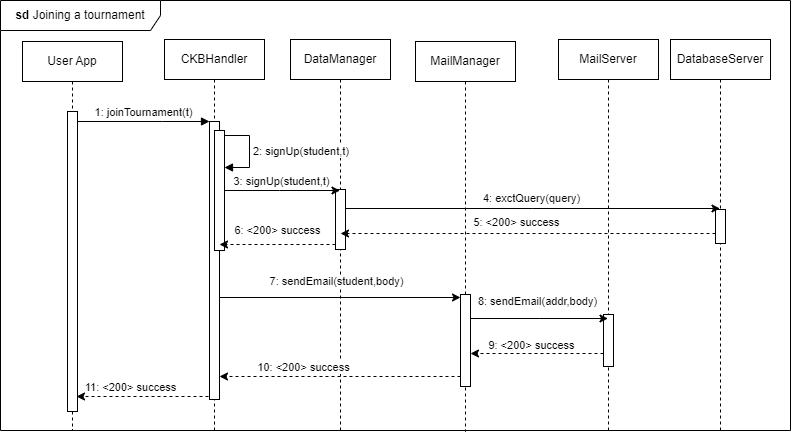
\includegraphics[width=1\textwidth]{images/seq_diagrams/joining_tournament_DD.png}
    \caption{Joining a tournament}
\end{figure}

\subsection{Joining a battle as a singleton}
The figure below shows a student joining a battle as a singleton and receiving an email notification about it.\\
\begin{figure}[H]
    \centering
    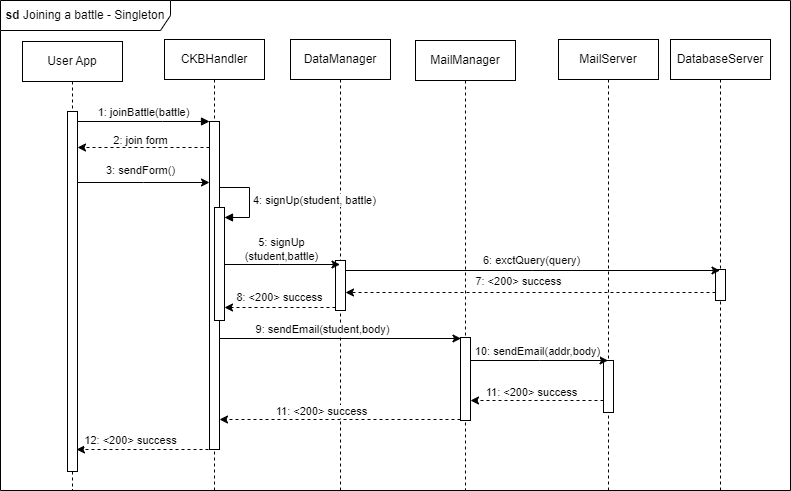
\includegraphics[width=1\textwidth]{images/seq_diagrams/joining_battle_singleton_DD.png}
    \caption{Joining a battle as a singleton}
\end{figure}

\subsection{Joining a battle by creating a group}
The figure below shows a student creating a group for a battle and receiving an email notification about it.\\
\begin{figure}[H]
    \centering
    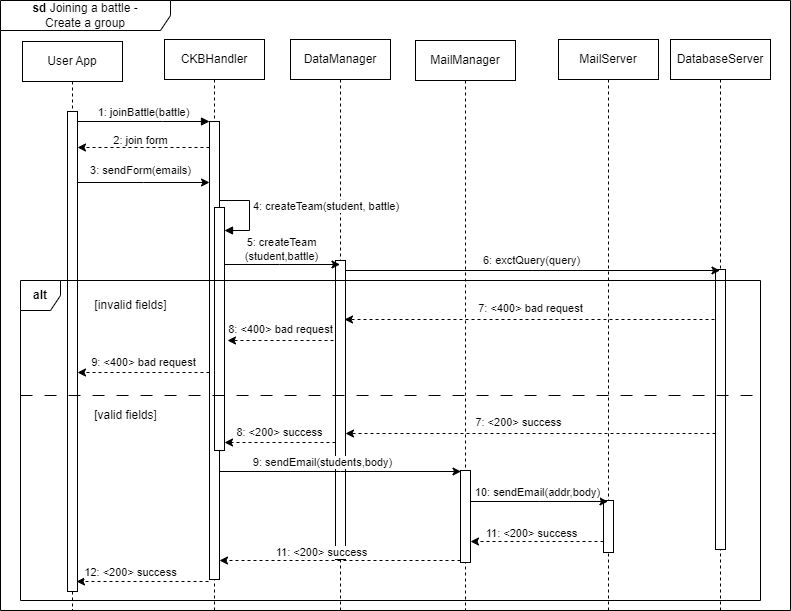
\includegraphics[width=1\textwidth]{images/seq_diagrams/joining_battle_create_group_DD.png}
    \caption{Joining a battle by creating a group}
\end{figure}

\subsection{Joining a battle by joining a group}
The figure below shows a student joining a group for a battle and receiving an email notification about it. If the 
minimum number of participants is reached, the team is signed up for the battle.\\
\begin{figure}[H]
    \centering
    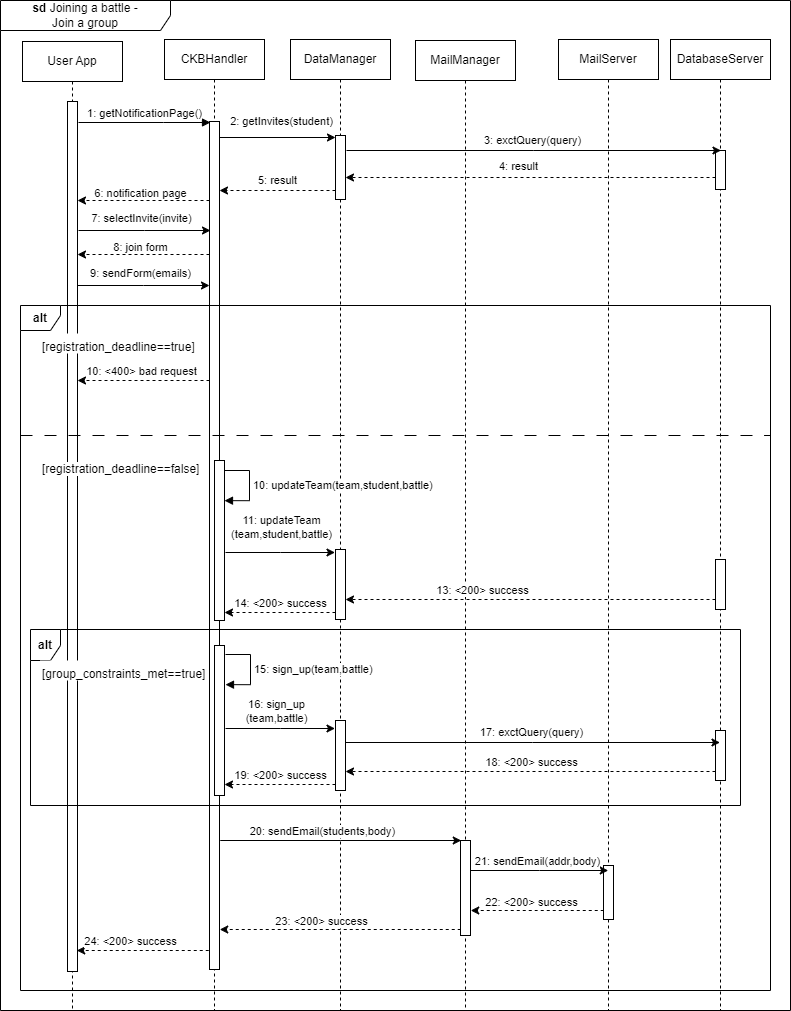
\includegraphics[width=1\textwidth]{images/seq_diagrams/joining_battle_join_group_DD.png}
    \caption{Joining a battle by joining a group}
\end{figure}

\subsection{Execution of the battle}
The figure below shows the sequence diagram of the execution of a battle. After GitHub notify the system that a student pushed code, the system
evaluate automatically the code based on the requirements chose by the educator at the creation of the battle and
updates the battle score of the student.
\begin{figure}[H]
    \centering
    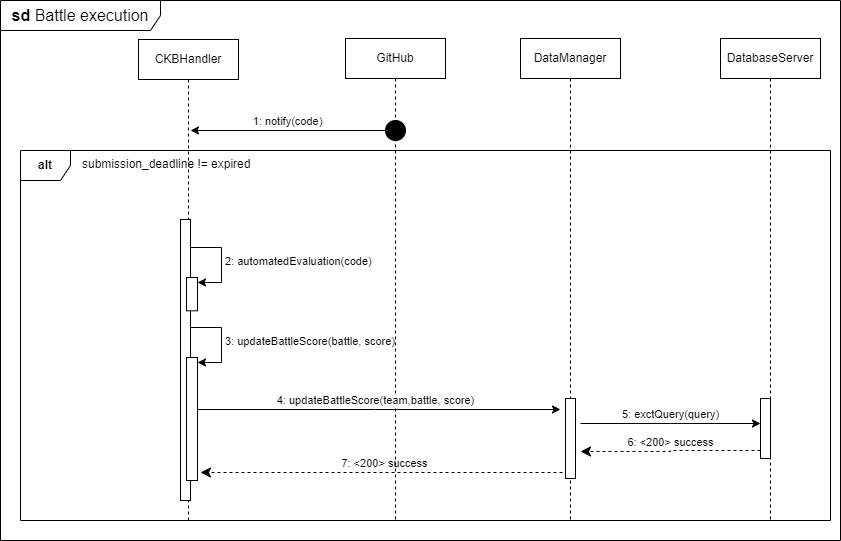
\includegraphics[width=1\textwidth]{images/seq_diagrams/battle_execution_DD.png}
    \caption{Execution of the battle}
\end{figure}

\subsection{Evaluation}
The figure below shows evaluation process of a students' solution: first the CKBHandler asks the EvaluationTool to evaluate the 
code according to the rules for automated evaluation, then, after the battle submission deadline expires and if required, the 
educator can manually evaluate the code.\\
\begin{figure}[H]
    \centering
    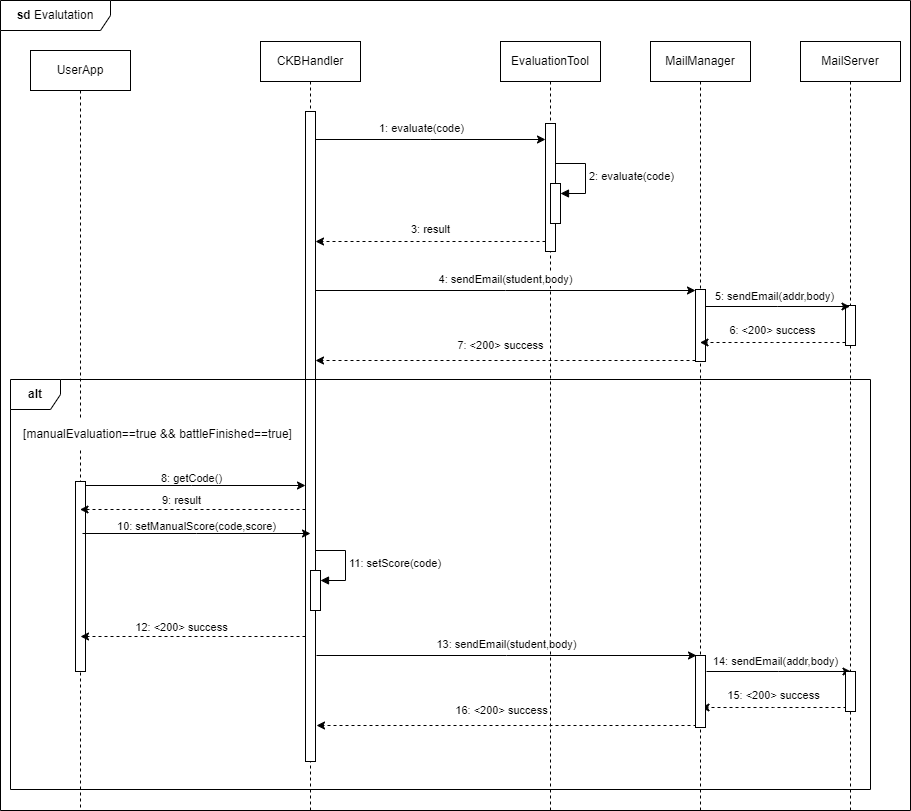
\includegraphics[width=1\textwidth]{images/seq_diagrams/evaluation_DD.png}
    \caption{Evaluation}
\end{figure}

\subsection{Conclusion of the battle}
The figure below shows the sequence diagram of the conclusion of a battle. The system updates the tournament
score of the students who participated to the battle and the tournament rank. The system send an email to all the students submitted
to the tournament to notify them that the updated tournament rank is available.
\begin{figure}[H]
    \centering
    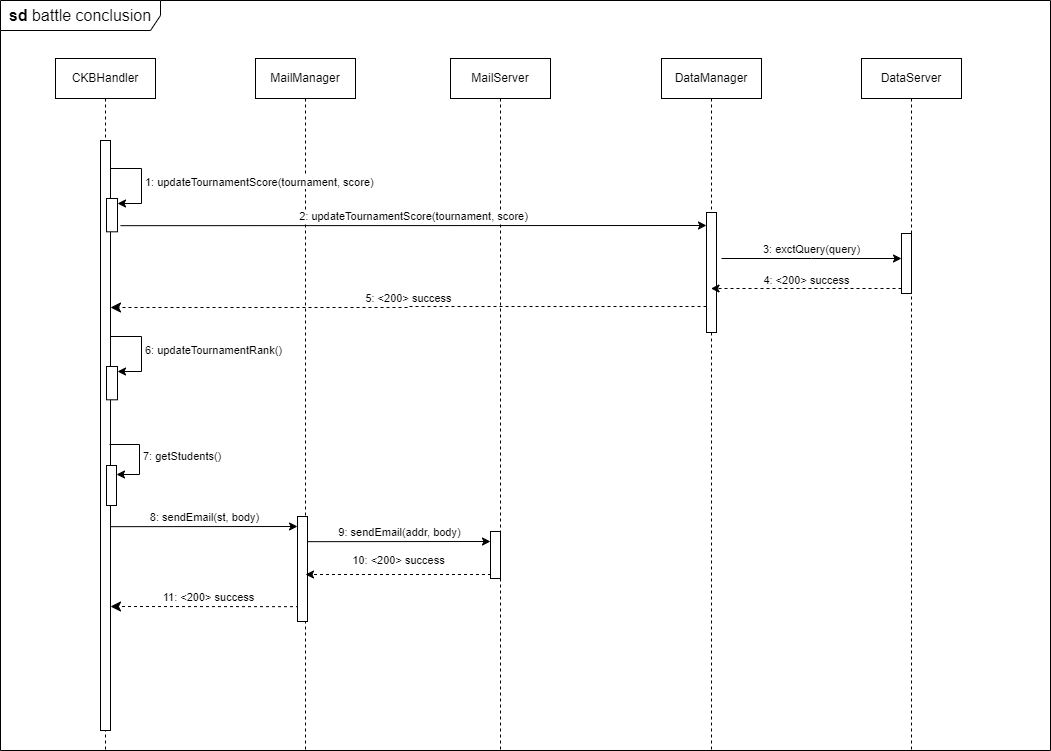
\includegraphics[width=1\textwidth]{images/seq_diagrams/battle_conclusion_DD.png}
    \caption{Conclusion of the battle}
\end{figure}

\subsection{Conclusion of a tournament}
The figure below shows the sequence diagram of the conclusion of a tournament. The educator chooses to conclude the tournament, so the system 
awards badges to students and sends an email notification to all suscribed students.
\begin{figure}[H]
    \centering
    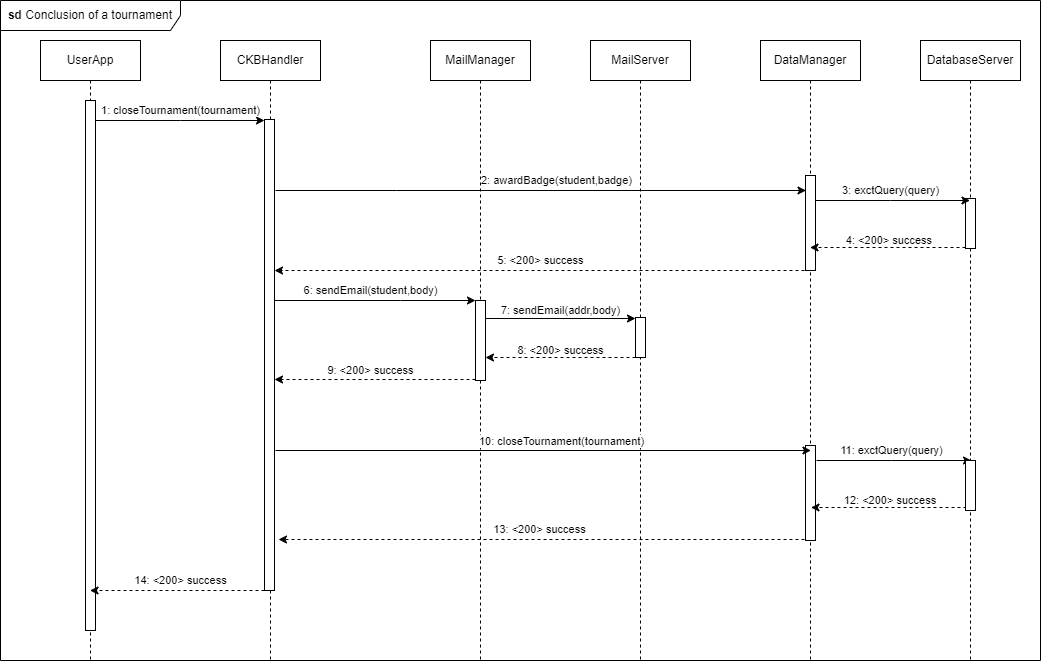
\includegraphics[width=1\textwidth]{images/seq_diagrams/tournament_conclusion_DD.png}
    \caption{Conclusion of a tournament}
\end{figure}

\subsection{Profile visualization}
The figure below shows the sequence diagram of the visualization of the profile of a student. 
The system retrieves the data of the seacrhed student from the database if the student is registered to the system, otherwise it sends an error message.
\begin{figure}[H]
    \centering
    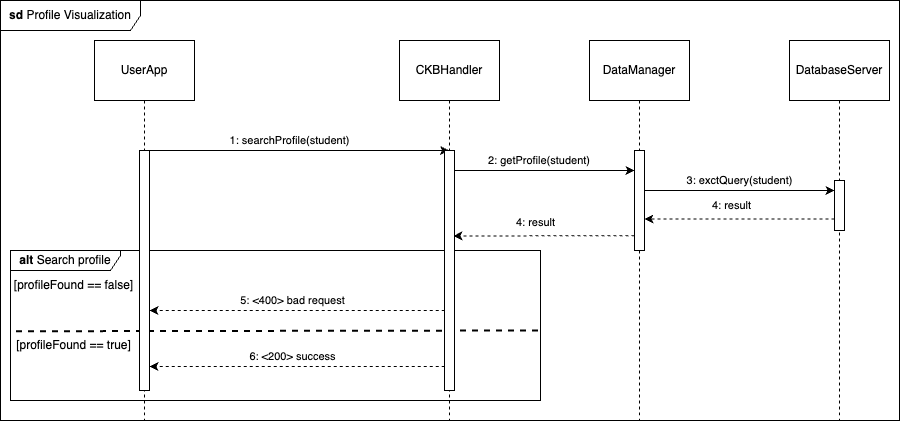
\includegraphics[width=1\textwidth]{images/seq_diagrams/ProfileVis_DD.png}
    \caption{Profile visualization}
\end{figure}

\section{Component interfaces}
In this section, the figure below depicts the interface diagram with the component interfaces and their specific methods and connections.
\begin{figure}[H]
    \centering
    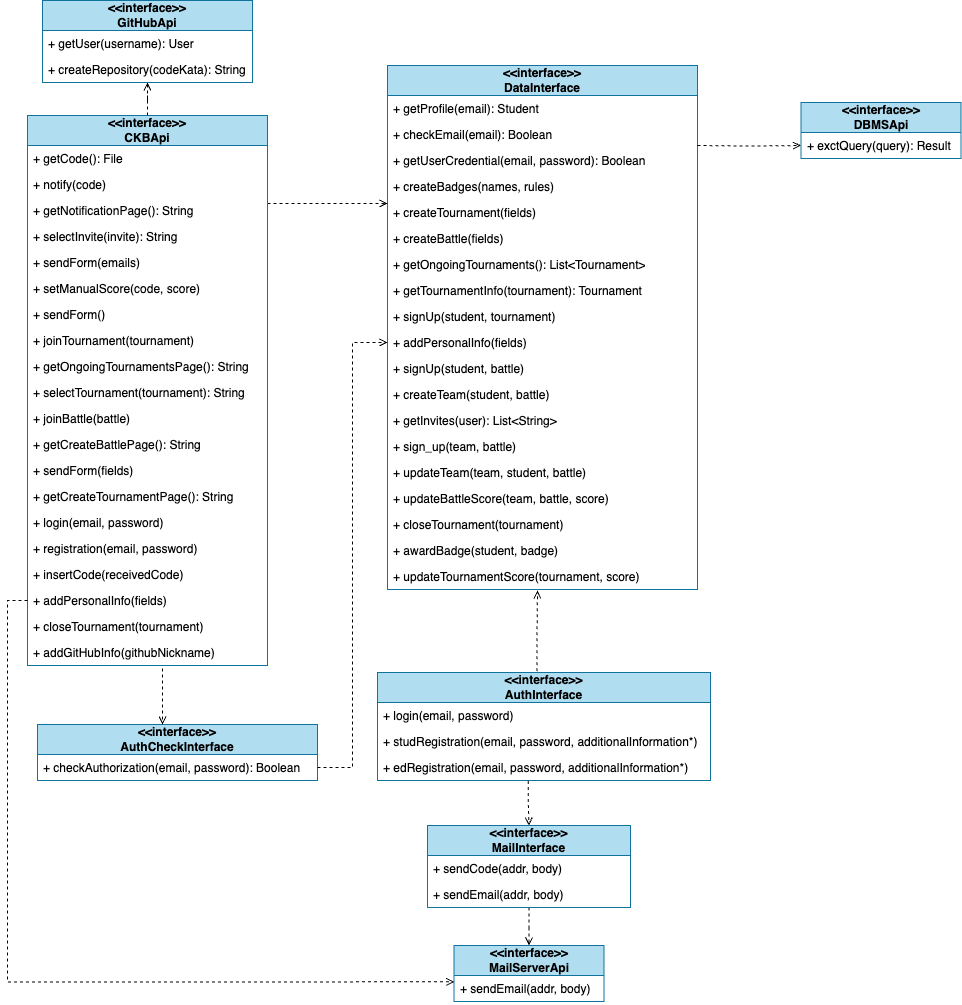
\includegraphics[width=1\textwidth]{images/Interface_diagram.png}
    \caption{Interface diagram}
\end{figure}

\section{Selected architetural styles and patterns}

\begin{itemize}
    \item \textbf{Three-layers architecture: }the system is based on a three-layers architecture, presentation, application and data layer. The separation of the layers
    allows to scale the application efficiently by distributing the workload across multiple servers. It also allows to improve the security of the system by protecting the data layer.
    It also improves the maintainability of the system by allowing to modify a single layer without affecting the other ones.
    \item \textbf{REST architectural style: }the system is based on the REST architectural style. REST is a software architectural style that defines a standard language for Web services. It is stateless and it makes easy
    to integrate with other systems thanks to the uniform interface. It also allows for a clear separation between the client and the server. Client are not concerned with the internal state of the server, promoting loose coupling
    and enhancing system maintainability.
\end{itemize}

\section{Other design decisions}

\subsection{ER diagram}
\begin{figure}[H]
    \centering
    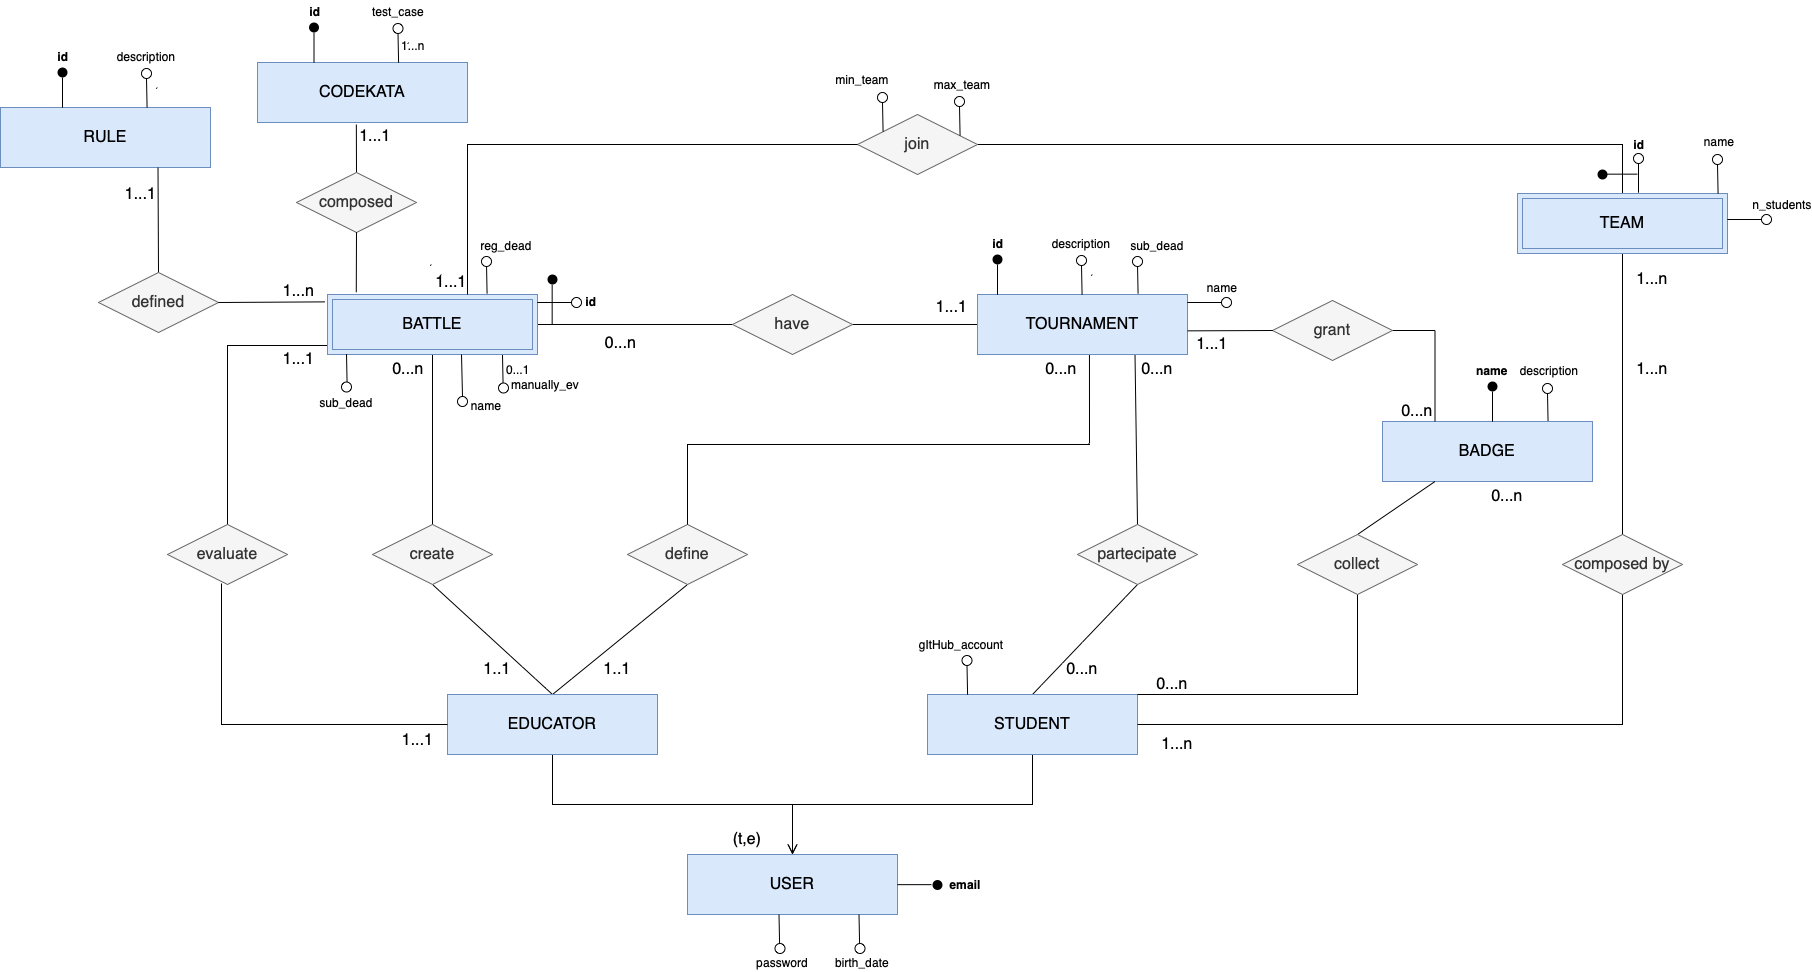
\includegraphics[width=1\textwidth]{images/ER_diagram.png}
    \caption{ER diagram}
\end{figure}